\vspace{10pt}

\minitoc
\clearpage

\section{Contexte de la thèse}
\subsection{Motivations}
% Introduction générale sur la robotique et sa progression
L'évolution de la robotique vers des usages de plus en plus transparents, proches du public et à grande échelle, ne fait guère de doute depuis plusieurs années. Certains besoins sont d'ores et déjà identifiés, tels les interventions dans des milieux hostiles ou l'assistance aux personnes, d'autres sont encore inespérés et seront sans doute popularisés dans les décennies à venir. Plusieurs aspects peuvent être moteurs pour favoriser cette évolution, des notions de confort, d'efficacité économique ou de sécurité par exemple.\\

% Importance du logiciel et des algorithmes dans l'évolution de la robotique
Les capacités matérielles accrues des plate-formes électroniques expliquent sans doute une partie de cette évolution, tant du point de vue des capteurs utilisés que des capacités de calcul. Les capteurs classiques, tels que les caméras, ont en effet fortement progressé ces dernières années, en termes de qualité comme de prix de revient. De nouveaux capteurs (perception en trois dimensions par exemple) sont par ailleurs apparus dans le grand public et autorisent de nouveaux usages. De même, les capacités de calcul en progression régulière depuis l'avènement de l'électronique grand public expliquent sans doute une partie de la progression des capacités des systèmes robotisés. Ceci ne représente cependant qu'une partie de leur évolution, tant l'état de l'art algorithmique a lui aussi évolué dans de multiples domaines.\\

%Importance du logiciel
Un système robotisé nécessite la prise en compte de plusieurs aspects, dont la perception de l'environnement, le contrôle de sa trajectoire, les communications ou la prise de décision. Les progrès dans ces domaines ont été très importants ces dernières décennies, et ne sont pas à sous-estimer lorsque l'on considère l'accroissement dans le même temps des capacités des engins autonomes. Les capacités matérielles doivent ainsi aller de pair avec un cadre algorithmique autorisant leur exploitation intelligente. Ces dernières décennies ont ainsi vu l'avènement d'algorithmes d'apprentissage, de reconnaissance, de cartographie et de localisation simultanées, qui correspondent à une exploitation nouvelle de capteurs existants. Il s'agit sans doute d'un aspect plus difficilement quantifiable, mais tout aussi important, que l'augmentation des performances de calcul. De nombreux travaux restent ainsi nécessaires pour augmenter les possibilités des systèmes autonomes, sans préjuger de leurs capacités matérielles.\\

% Contexte global de la thèse : déplacement autonome
Les domaines d'étude sont donc nombreux, et ce manuscrit n'a pas l'ambition d'en réaliser une étude exhaustive. Il s'inscrit plus particulièrement dans la problématique des véhicules ou robots se déplaçant de manière autonome, et s'intéresse plus spécialement aux besoins liés à la perception de l'environnement, que nous détaillerons par la suite. Il s'agit schématiquement d'acquérir des informations sur le contexte dans lequel le véhicule évolue, qui peuvent ensuite être exploitées pour alimenter les algorithmes de planification et d'intelligence artificielle.

\subsection{IMARA}
L'équipe IMARA (\emph{Informatique, Mathématiques et Automatique pour la Route Automatisée}) est présente au centre INRIA de Rocquencourt depuis 2008, elle fait partie du consortium LaRA (\emph{La Route Automatisée}, comprenant le laboratoire CAOR des Mines Paristech et le laboratoire LIVIC) visant à l'étude et au développement de moyens technologiques d'automatisation des moyens de transport. Il s'agit d'une équipe transversale, dans le sens où plusieurs domaines de recherche sont abordés, tels que le contrôle, la communication, la modélisation des réseaux de transport ou la perception de l'environnement. L'équipe compte notamment 9 membres permanents, 14 chercheurs et 5 thésards. Les véhicules d'expérimentation sont des automobiles grand public équipées pour la recherche (Citroën C3 et C1), ainsi que des véhicules automatisés disposant de caméras et de télémètres laser à balayage (de type \emph{CyCab} et \emph{CyBus}, cf. figure \ref{fig:ch1_IMARA}).

\begin{figure}
	\centering
	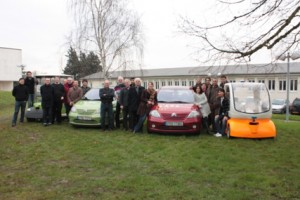
\includegraphics[width=0.7\textwidth]{Chapter1/graphics/imara.jpg}
	\caption{L'équipe-projet IMARA et quelque uns des véhicules utilisés}
	\label{fig:ch1_IMARA}
\end{figure}

\subsection{Perception de l'environnement : quels besoins pour une navigation autonome ?}
\subsubsection{Définition}
On parlera souvent dans ce manuscrit de "<perception de l'environnement\fg{}, et cette notion peut être diversement comprise. Ce premier paragraphe sera donc l'occasion d'une définition, à laquelle nous tâcherons de nous tenir par la suite. On appelle donc ici \emph{perception de l'environnement} l'action d'acquérir des informations, de quelque nature que ce soit, sur les éléments constitutifs de l'espace à proximité du porteur. Ces éléments peuvent être de nature structurelle (route, bâtiments, objets rigides, ..) ou immatérielle (position par rapport à un référentiel donné, ..), ils peuvent être constants dans le temps ou dynamiques (leur caractéristique, par exemple leur position, change avec le temps). \\
Ces informations sont très diverses par nature, et peuvent donc prendre des représentations différentes, nous en détaillerons quelques unes dans la section \ref{sec:ch2_capteurs}.

\subsubsection{Besoins de perception pour un véhicule autonome} \label{sec:ch1_besoins}
Un véhicule autonome doit, par définition, être capable de percevoir toutes les informations nécessaires à une navigation sans incident ; que ce soit vis-à-vis d'autrui (collision avec un élément de la scène) ou de son intégrité propre. Il doit par ailleurs être capable de communiquer avec son environnement dans de nombreux cas de figure, pour coordonner son action avec d'autres porteurs ou recevoir de nouvelles informations ou directives par exemple. Il doit enfin être capable de prendre des décisions et de planifier des actions de manière indépendante, ce qui implique d'acquérir préalablement suffisamment d'informations sur son environnement.\\

On peut ainsi sommairement lister quelques uns de ces besoins concrets liant un véhicule autonome et son environnement, indépendants de la représentation utilisée ou des capteurs :
\begin{itemize}
	\item perception des obstacles statiques;
	\item positionnement dans l'espace par rapport à l'environnement courant;
	\item positionnement dans l'espace par rapport à une référence absolue;
	\item détection, localisation, suivi des objets en mouvement;
	\item perception de l'espace navigable;
	\item perception de symboles porteurs de sens (panneaux, signalisation routière, ou autre).\\
\end{itemize}

Certains de ces éléments peuvent être résolus par une connaissance \textit{a priori} de la scène, et la notion de perception doit donc être comprise au sens large (acquisition d'information). On peut aisément constater que les besoins sont nombreux, bien que certains d'entre eux soient résolus depuis plusieurs années dans certaines conditions favorables. Nous n'avons pas l'ambition de répondre à tous ces besoins par la méthode présentée dans ce manuscrit, mais nous concentrerons sur quelques points particuliers.

\subsection{Buts poursuivis}
Notre travail se situe dans le domaine des véhicules autonomes, et concerne de manière plus générale tous les robots amenés à se déplacer dans un environnement dynamique. Nous souhaitons améliorer les capacités de perception des obstacles et des objets mobiles, et être capable d'estimer leurs caractéristiques dynamiques (vitesse et direction). Ces besoins sont par exemple nécessaires à l'évolution de robots dans un environnement partagé avec des humains, et constituent l'un des axes de progrès majeurs dans le domaine de la perception. Une grande proportion des algorithmes couramment utilisés pour la navigation des véhicules autonomes suppose en effet que l'environnement observé est statique, et que les éléments mobiles sont assimilables à un bruit d'observation. La connaissance de la vitesse des éléments mobiles de l'environnement autorise au contraire une planification de trajectoire plus sûre et efficace, en autorisant notamment une anticipation inaccessible aux moyens de perception restreints à un monde statique.\\

Les buts poursuivis peuvent être résumés par les quatre points suivants :
\begin{itemize}
	\item{\emph{Localisation autonome du porteur dans son environnement proche:}\\}
	La méthode proposée doit être capable d'estimer la position et le mouvement du véhicule de manière autonome, c'est à dire sans faire appel à des capteurs ou à des moyens de calcul externes.\\
	
	\item{\emph{Positionnement des obstacles statiques dans l'espace:}\\}
	La méthode proposée doit pouvoir servir de base à une détection des obstacles, ce qui suppose donc que suffisamment de points de la scène soient positionnés dans l'espace pour ne pas risquer une collision. La classification des éléments de la scène n'est cependant pas l'objet de ce travail, mais nous souhaitons obtenir les informations suffisantes pour répondre à ce besoin.\\
	
	\item {\emph{Détection des objets mobiles, de leur position et de leur vitesse:\\}}
	La méthode que nous présentons vise à détecter les objets se mouvant indépendamment du porteur, et à estimer leur position et leur vecteur vitesse. Ces informations sont utiles pour la planification de trajectoire du véhicule, et une classification postérieure de ces objets en tant qu'obstacles potentiels.\\
	
	\item{\emph{Exécution en temps réel:}\\}
	Les tâches liées à la navigation d'un véhicule autonome sont naturellement soumises à des contraintes en termes de temps de calcul. On peut se convaincre empiriquement que ces contraintes sont de l'ordre des temps caractéristiques de la dynamique du porteur (temps nécessaire pour revenir à l'immobilité notamment), que l'on résumera improprement dans la suite par \og \textit{temps réel} \fg. Cette définition n'est pas stricte dans notre cas, s'agissant de temps d'exécution qui peuvent varier selon la plate-forme de calcul notamment, mais on s'attachera à montrer que leur ordre de grandeur est adaptée à une acquisition continue d'informations visuelles, soit environ 10 à 25 images traitées par seconde.\\
\end{itemize}

\section{Organisation du manuscrit}
Le chapitre 2 est dédié à un état de l'art des systèmes de perception répondant à notre problématique. Il s'agit tout d'abord de présenter différents capteurs à même de répondre à notre problématique, ainsi que certains des algorithmes qui y sont associés dans la littérature et qui répondent à tout ou partie des besoins soulevés. Ces approches ne satisfont pas tous nos prérequis, et on proposera alors un mécanisme général visant à y répondre.\\

Le chapitre 3 sera consacré à l'acquisition d'informations à partir de capteurs d'imagerie, et au type d'information que nous souhaitons obtenir. On présentera initialement quelques uns des algorithmes présents dans l'état de l'art qui visent à exploiter des acquisitions visuelles à des fins de perception. On présentera ensuite le type d'information que nous avons souhaité utiliser, ainsi qu'une évaluation quantitative de différentes approches s'y rattachant. On présentera ensuite une implémentation très parallélisée que nous avons réalisé afin d'assurer un traitement rapide de cette étape de l'algorithme.\\

Le chapitre 4 présente une partie du processus d'inférence se basant sur les indices visuels, qui répond à une problématique d'odométrie visuelle et de reconstitution de l'environnement statique autour du porteur. On présentera une nouvelle méthode proposée pour estimer de manière rapide et robuste le mouvement, qui s'adapte aux informations visuelles ponctuelles extraites lors de l'étape précédente, et qui sera comparée à l'état de l'art. Le mécanisme proposé pour estimer la position dans l'espace d'éléments singuliers de l'environnement sera également présenté, ainsi que quelques résultats spécifiques à cette étape de l'algorithme.\\

On présente ensuite dans le chapitre 5 la détection et le suivi des objets mobiles, qui sont aussi obtenus à partir des informations extraites des acquisitions visuelles. Différentes méthodes de détection d'objets mobiles sont initialement présentées, puis nous détaillons notre proposition qui prend en compte les spécificités de notre système d'acquisition. De même, on présentera dans cette partie quelques méthodes présentes dans la littérature permettant l'estimation de la localisation et le suivi de cibles mobiles, avant de détailler l'approche que nous proposons et de commenter les résultats obtenus.\\

Le chapitre 6 est enfin consacrée à une illustration des résultats généraux de la méthode proposée, et une critique relative à son adéquation aux problématiques initiales. Nous proposerons alors quelques pistes d'amélioration des travaux existant, avant de conclure ce manuscrit.

\section{Contributions}
On propose dans ce manuscrit les contributions suivantes :
\begin{itemize}
\item Système global de perception d'un environnement dynamique, fournissant un nuage de points semi-dense suivi dans le temps. Il s'agit d'une approche globale et novatrice, qui est focalisée sur nos besoins en termes de perception des objets mobiles.\\

\item Détermination du mouvement propre de la caméra (\emph{Ego-motion}) dans un cadre adapté aux spécificités de la stéréo-vision. Il existe dans ce domaine une littérature abondante, qui n'est cependant pas toujours adaptée à nos besoins. On propose une méthode rapide et robuste qui répond très bien à notre problématique initiale.\\

\item Détection et suivi d'objets mobiles dans l'espace. On propose un système novateur, à même de détecter et d'estimer la position et la vitesse d'éléments mobiles de la scène, sans prérequis de forme ou de trajectoire, à partir d'acquisitions visuelles.
\end{itemize}